\subsection{Algorithme de Toussaint}
Cet algorithme est basé sur le constat suivant : un des côtés du rectangle minimum doit être colinéaire à l'un des côtés de l'enveloppe convexe. De ce fait, l'algorithme proposé par Godfried Toussaint en 1983 consiste en la recherche de tous les rectangles possibles vérifiant la proposition précédente puis de retenir celui dont l'aire est la plus petite.

Le point délicat de l'implantation de cet algorithme est la bonne gestion de la rotation du rectangle sur les faces de l'enveloppe convexe. Une bonne méthode est de se servir de la technique du \og pied à coulisse \fg{} donnée par Michael Shamos en 1978.

\begin{figure}[ht]
\begin{center}
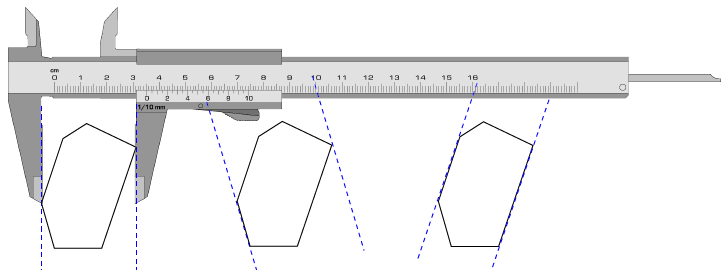
\includegraphics[scale=0.6]{images/shamos.png}
\caption{Technique du pied à coulisse}
\end{center}
\end{figure}

Le point de départ est de construire un rectangle passant par les point cardinaux du plan, autrement dit par les points d'abscisse minimum et maximum ainsi que d'ordonnée maximum et minimum. Cette étape est de complexité linéaire $\mathcal{O}(n)$. On rappelle que l'algorithme de Toussaint implique d'obtenir l'enveloppe convexe au préalable.
A présent, il suffit de nous servir de 2 pieds à coulisse ($NORD-SUD$ et $OUEST-EST$) pour construire les rectangles encadrant notre ensemble de points : puisque le rectangle de départ à été construit à partir des points cardinaux de notre ensemble, tous les points sont nécessairement contenus dans ce rectangle.

Pour savoir de quelle manière est-ce que nous allons faire tourner nos pieds à coulisse il nous faut calculer les angles formés par les côtés du rectangles et les faces de l'enveloppe convexe pour un total de 4 angles $\theta _i$, $\theta _j$, $\theta _k$ et $\theta _l$. A partir de ces angles, nous faisons tourner le rectangle d'un angle $min\{\theta _i, \theta _j, \theta _k, \theta _l\}$.

\newpage
\begin{figure}[ht]
\begin{center}
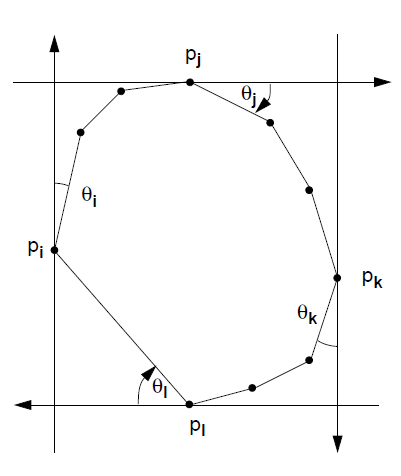
\includegraphics[scale=0.5]{images/toussaint.png}
\caption{Algorithme de Toussaint}
\end{center}
\end{figure}

Une des conditions d'arrêt, plutôt que de traiter toutes les faces possibles de l'enveloppe convexe, serait de s'arrêter lorsque le rectangle aura tourné à plus de $90$\degre ce qui signifierait que nous sommes retombés dans le cas du rectangle initial.

\begin{figure}[ht]
\begin{center}
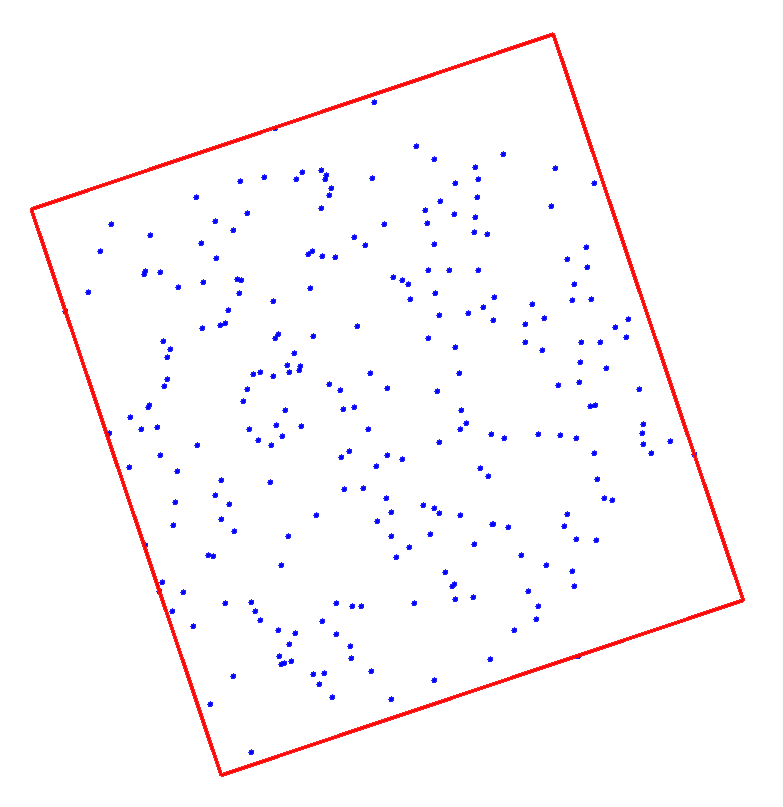
\includegraphics[scale=0.25]{images/ex_toussaint.png}
\caption{Exemple d'application Toussaint}
\end{center}
\end{figure}

Il reste ensuite à calculer l'aire de tous les rectangles obtenus qui peut se faire en temps constant $\mathcal{O}(1)$ (la formule de l'aire d'un polygone convexe peut être utilisée ici et sera décrite dans la partie \ref{efficacite}) pour une complexité totale de $\mathcal{O}(n)$.

Finalement, l'algorithme de Toussaint, bien que les étapes sont au plus de complexité linéaire, est de complexité pseudo-linéaire en $\mathcal{O}(n\log{n})$ car majoré par le calcul de l'enveloppe convexe qui est pseudo-linéaire.
\newpage